\section{Project management methodologies}
\label{ProjMgmtMethods}
This section details how the different teams manage themselves. This is done for reasons of transparency, so that the reader understands which project management methods the individual teams use. This highlights an additional level of complexity in the working environment. Not all teams are addressed in every subsection, as the project team was not involved in all teams’ methods to the same depth. First, project management methods are highlighted, followed by the different timeline management approaches. In the following figure, the different boards and management methods are aligned around the central academic team to illustrate the broad set of methods.

\begin{figure}[H]
    \centering
    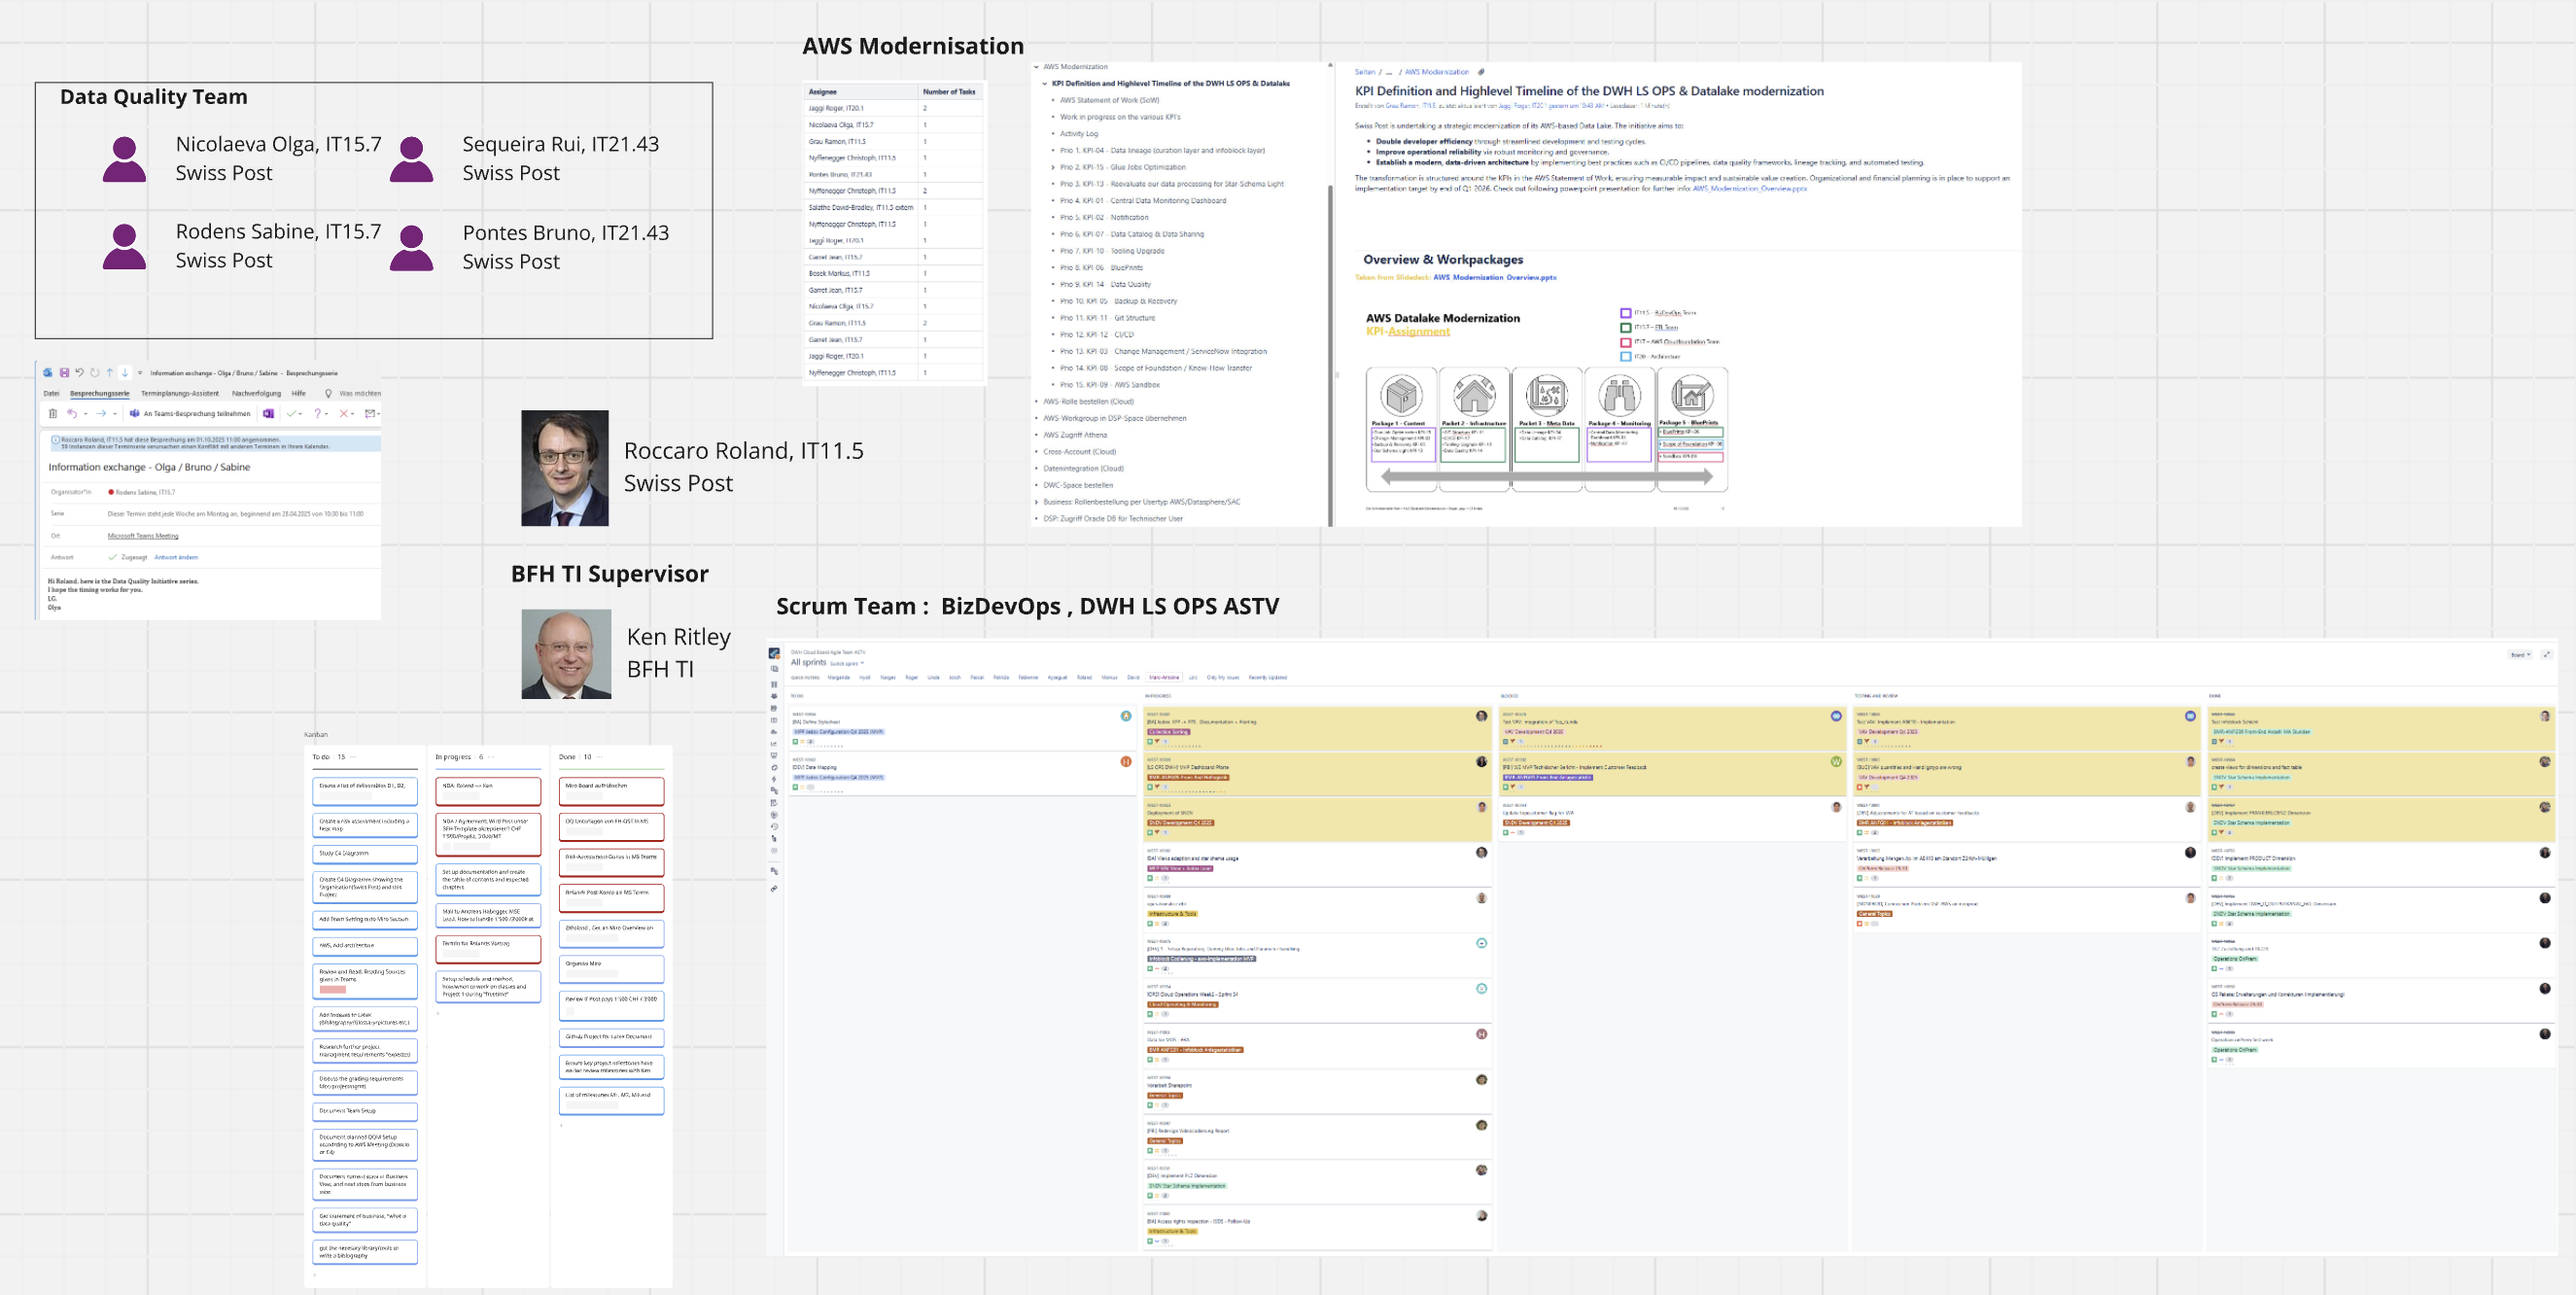
\includegraphics[width=0.8\textwidth]{./content/img/PostTeams_Tools.png}
    \caption{All methods on one picture showing their diversity}
    \label{fig:projmgmt_methods_one_pic}
\end{figure}

\subsection*{Project management}
Project management for this project consists of three main elements. These are Scrum, Kanban, and weekly meetings.

\subsubsection*{Scrum}
The \gls{DWHLSOPS} team is organised as a \gls{BizDevOps} \gls{scrum} team (see Section \ref{sec:DWHLSOPSTeam}). The AWS modernisation teams join these Scrum teams \ref{sec:AWSmodernisationteam}. The full set of rituals defined for Scrum is used, including daily meetings, sprint retrospectives, sprint planning held every two weeks, and reviews held every four weeks. In addition, a weekly Scrum meeting is held to maintain communication between the ASTV, D\&F, and MPP teams. The meetings are shown in the first screenshot, while the second illustrates a noteworthy team definition: the rules of engagement established for collaboration, which are a result of the retrospectives.


\begin{figure}[H]
    \centering
    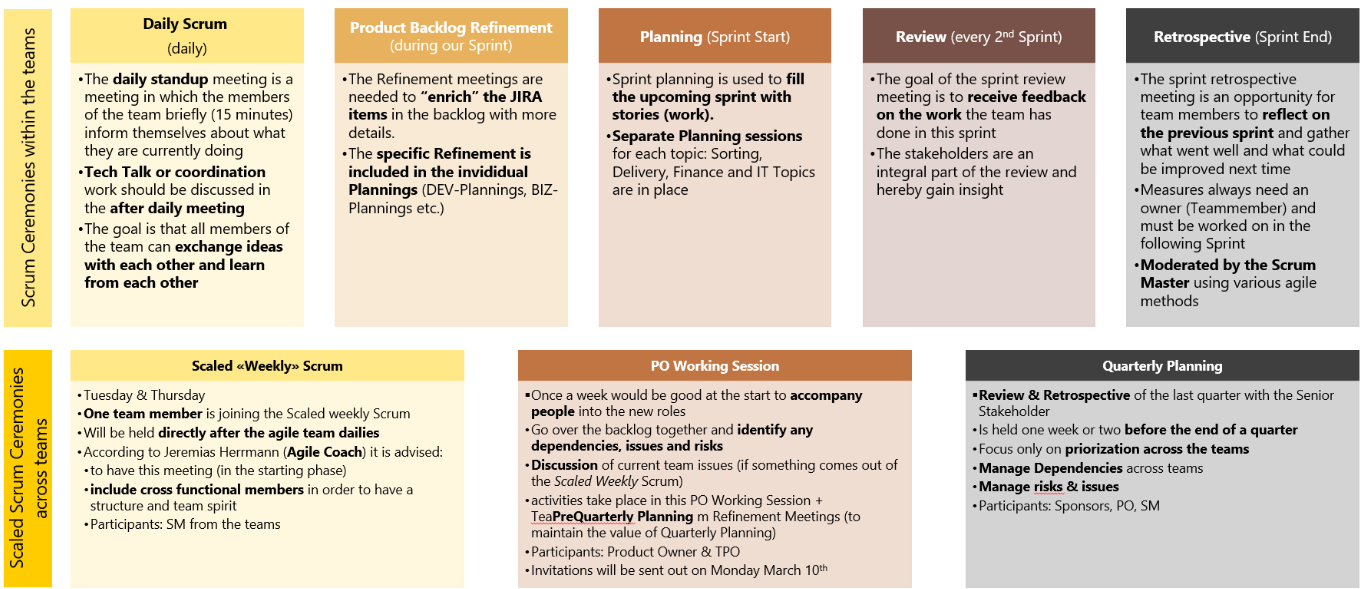
\includegraphics[width=0.8\textwidth]{./content/img/ProjectManagement/BizDevOps_ScrumCeremonies.PNG}
    \caption{Scrum ceremonies of DWH LS OPS  BizDevOps team}
    \label{fig:projmgmt_bizdevops_scrumMeetings}
\end{figure}

\begin{figure}[H]
    \centering
    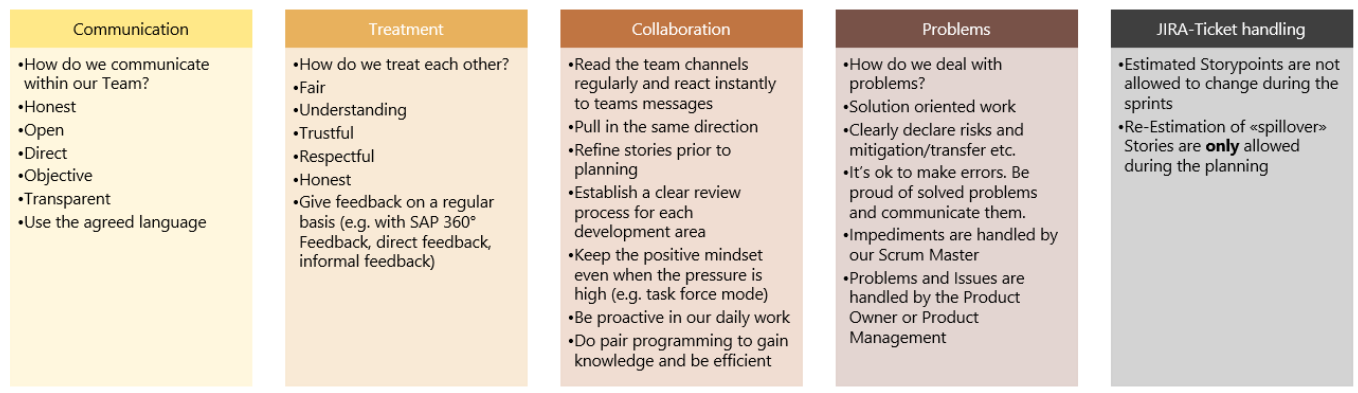
\includegraphics[width=0.8\textwidth]{./content/img/ProjectManagement/BizDevOps_RulesOfEngagement.png}
    \caption{Rules of engagement of DWH LS OPS  BizDevOps team}
    \label{fig:projmgmt_bizdevops_rulesofengagement}
\end{figure}

\subsubsection*{Weekly Meetings}
Contact with the \gls{DQM} team is handled using weekly meetings \ref{sec:DQMteam}. These serve as minimal update sessions during which weekly progress is communicated to all team members. While the developers in the DQM team are themselves also part of a Scrum team, their sprint management is out of scope.

\subsubsection*{Kanban}

The academic team handles tasks using a \gls{kanban} board \ref{sec:AcademicTeam}. The tasks are organised into three main columns. Both team members show their responsibilities on the Kanban board. The blue cards represent the author’s tasks, while the red cards represent the advisor’s tasks. The board is updated frequently and is reviewed during the weekly Jour Fixe.

\begin{figure}[H]
    \centering
    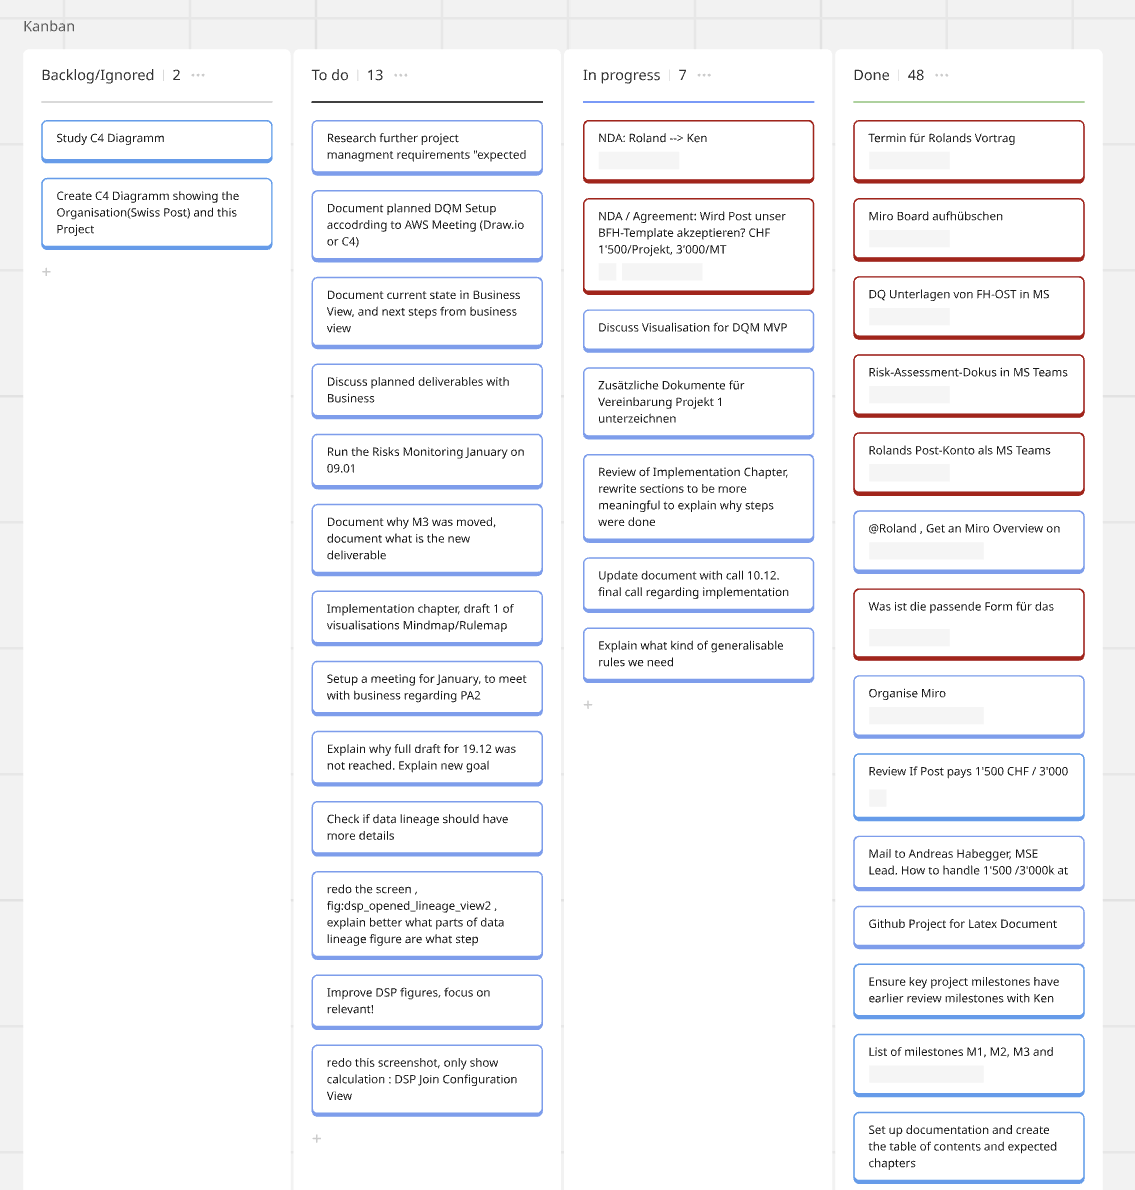
\includegraphics[width=0.8\textwidth]{./content/img/ProjectManagement/Academic_Kanban.png}
    \caption{Kanban board of Academic team}
    \label{fig:projmgmt_academic_kanban}
\end{figure}

\subsubsection*{Jour Fixe}

The academic team holds a \gls{JourFixe} every week \ref{sec:AcademicTeam}. This serves to maintain close communication and functions as a check-up meeting. Each meeting follows a defined structure; as an example, the meeting held on 15.12.2025 is described below.

\begin{itemize}
    \item Project check-in and clarification of objectives
    \item Overview of the project and completed deliverables
    \item Current deliverable in progress
    \item Status of milestones
    \item Changes needed to the updated Project 1 description
    \item Questions regarding Project 2
    \item Other topics
\end{itemize}

First, a general introduction to the project is provided to serve as a check-in and to allow participants to focus on the project. Second, the deliverables currently being worked on are listed based on the deliverables overview. Third, the status of the milestones is reviewed. Fourth, this is followed by individual agenda items, which can differ from meeting to meeting. In this meeting, these included updates to the Project 1 description required for agreement, as well as a check-in regarding topics and submission of Project 2. Finally, the meeting is closed with an open section in which any other relevant topics may be discussed. These meetings are documented in Miro (see below) and structured using a three-block template and are most often recorded using handwritten notes that are later uploaded.


 \begin{figure}[H]
    \centering
    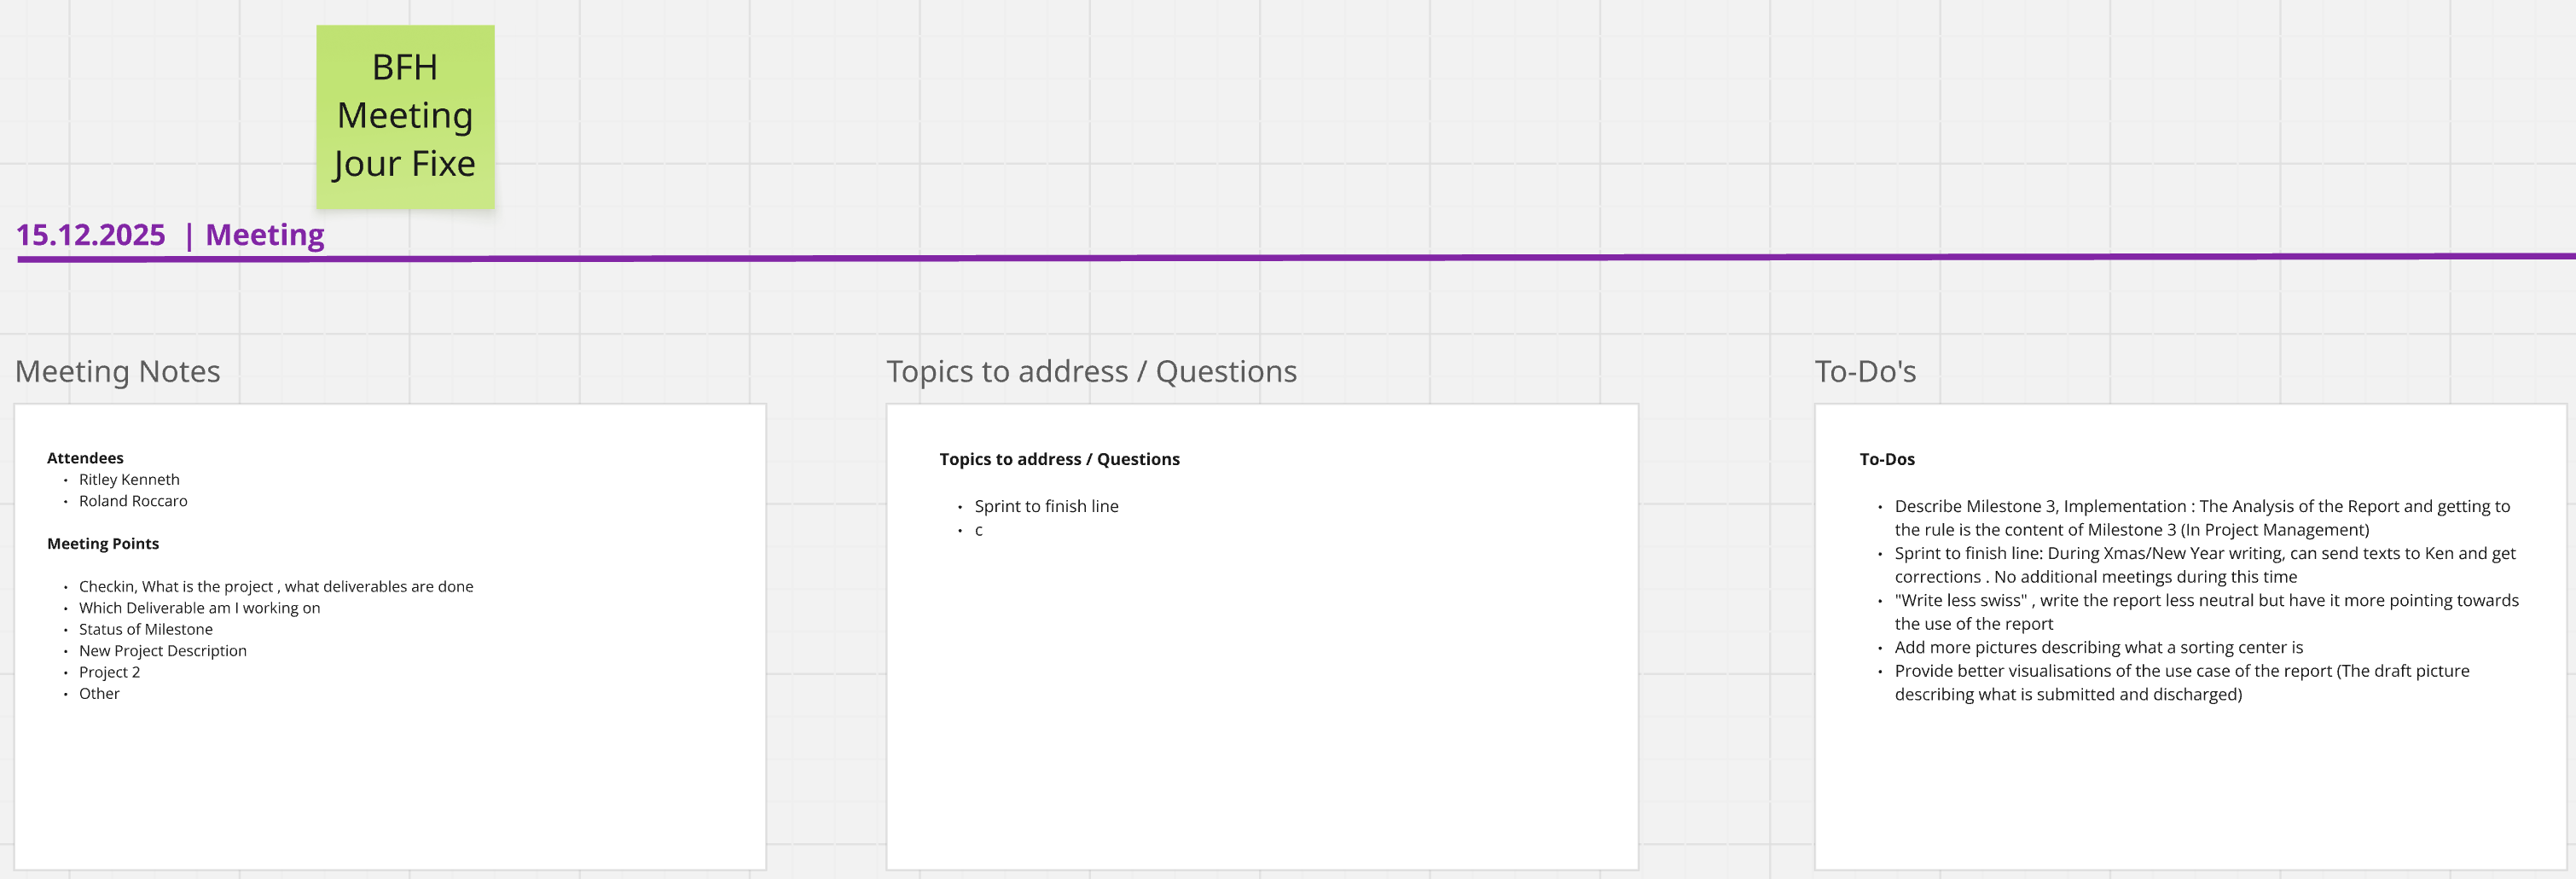
\includegraphics[width=0.8\textwidth]{./content/img/ProjectManagement/Academic_JourFixe.png}
    \caption{Jour Fixe of Academic team, meeting structure and rework}
    \label{fig:jour_fixe_academic_structure}
\end{figure}

\begin{figure}[H]
    \centering
    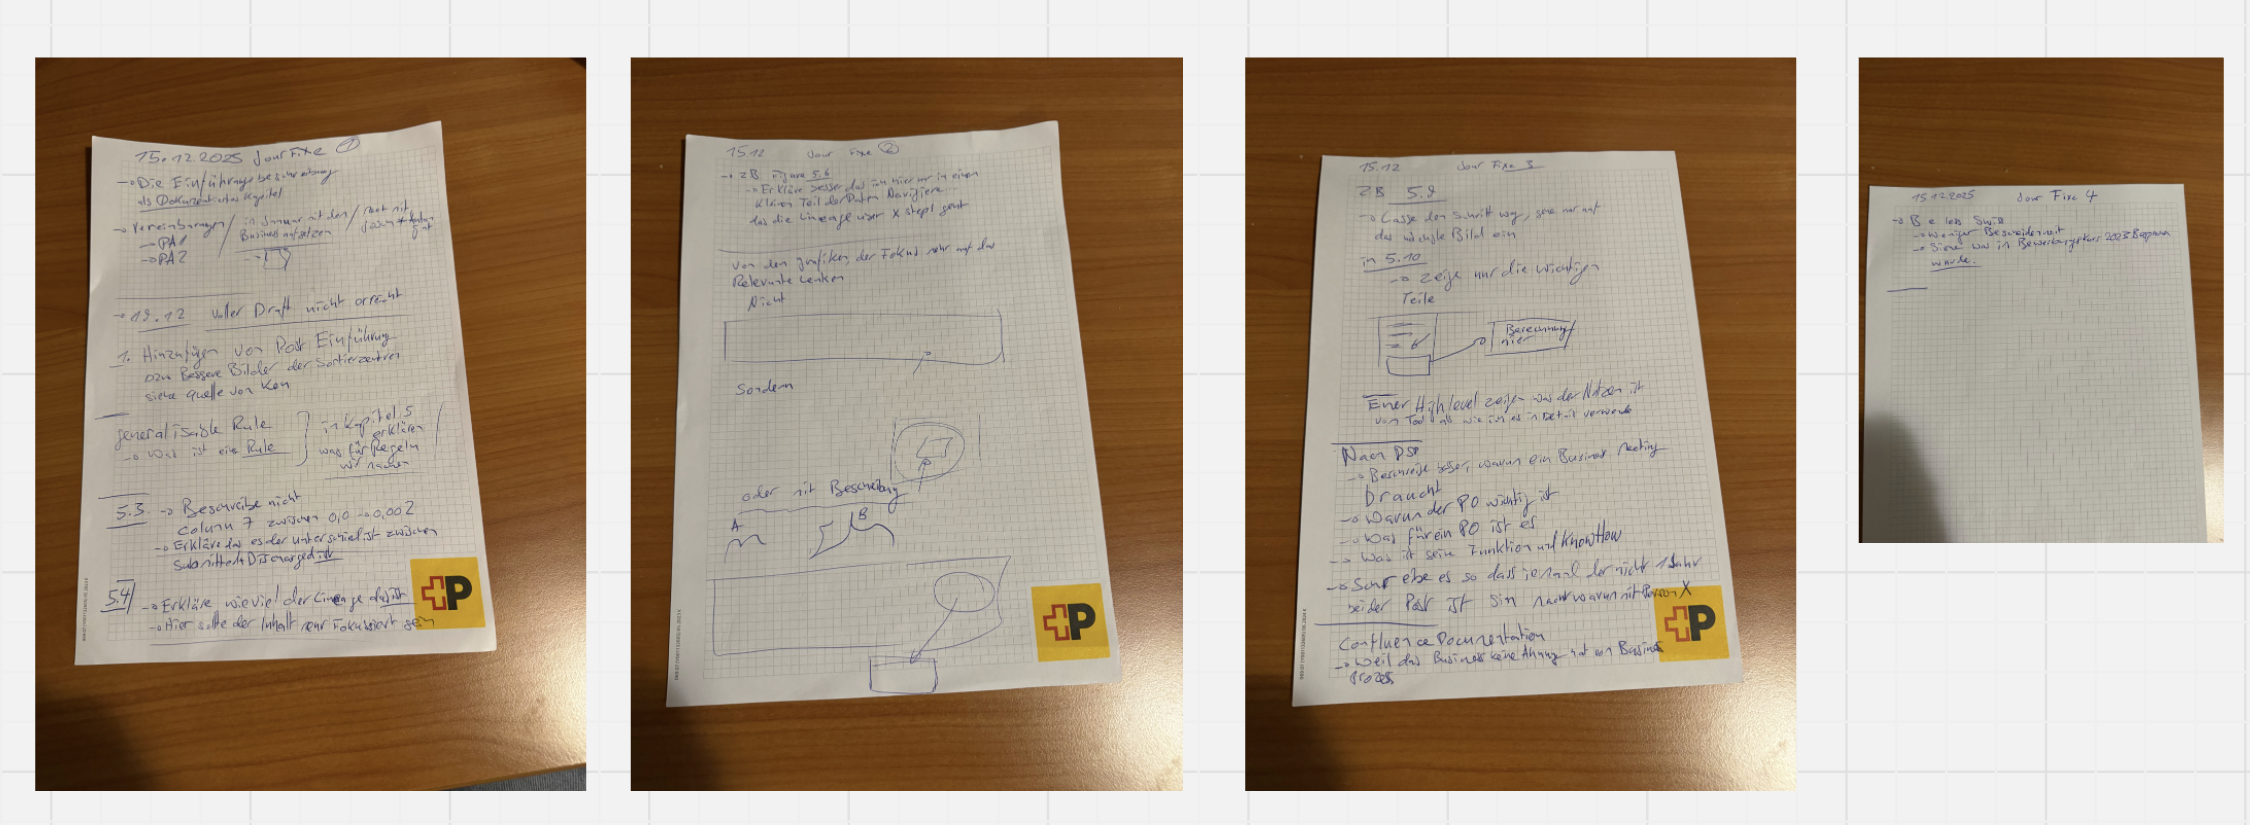
\includegraphics[width=0.8\textwidth]{./content/img/ProjectManagement/Academic_Jour_Fixe_Notes.png}
    \caption{Jour Fixe documentation of Academic team}
    \label{fig:jour_fixe_notes_academic}
\end{figure}

\subsection*{Timeline management}
Timeline management is performed in different ways by the teams. In this subsection, the planning of actions is described, as well as how staff availability is tracked.

\subsubsection*{Scrum Events}
The DWH LS OPS and the AWS modernisation teams use Scrum events to manage their timelines. Progress on stories is monitored in daily meetings, during which each team member updates the team on progress and issues and indicates whether assistance is needed or deviations from the previously planned approach are required. Sprints encompass the stories the team works on during a two-week cycle. During sprint planning, the stories for the next sprint are defined. The stories added to a sprint represent the commitment the team makes for the sprint, together with the sprint goal. Planning over longer time horizons is conducted through quarterly planning sessions. Every three months, all teams in DWH LS OPS plan which \gls{epic}s and how many story points should be completed. These quarterly planning sessions also serve to prioritise epics and allow higher management to introduce priorities.

\subsubsection*{Holidays}
Holidays are noted in the calendars used; this applies to the DWH LS OPS team as well as the academic team. In both cases, every holiday must be recorded with an absence notification. This allows other team members to quickly see whether a team member is available in the future and to adjust their planning accordingly, or to confirm in daily operations that the person is not available.

\subsubsection*{Milestones}
The academic team manages the planning of the overall project timeline using milestones. These milestones define timeframes during which a section or chapter may be worked on. For this project, the following milestones have been defined:

\begin{itemize}
    \item Milestone 1: Basics completed
    \item Milestone 2: Completion of main research
    \item Milestone 3: Code implementation completed
    \item Milestone 4: Bug fixing completed
    \item Milestone 5: Submission of the project document
    \item Milestone 6: Presentation prepared
\end{itemize}

First, the basics ready refers to tools to work with beeing available. This step includes setting up LateX, setting milestones, setup of basic tool structure and definition of way of work. Second the main research done refers to the end of the purely theoretical part and start towards the solution design and the subsequent implementation of it. This comprises the main literature research beeing done. Third, the code done refers to the implementation of the solution beeing done. After this point no new features are to be implemented. Fourth, bug fix done comprises all corrections that had to be performed so that the provided implementation works and technical debt amassed during development has been cleared. Fifth, the handin of the document is the final day according to the semester calender. Up to this date corrections to the document and finalisation can be provided. Sixth and final, the presentation must be ready latest by this date. After this some finetuning can be performed but the main content needs to be set.

The milestones were set to structure the work blocks, but primarily to define how much effort should be invested in each individual block. The time allocated per block is not estimated in terms of how long a task is expected to take. Instead, it is defined by how much time the team is willing to invest in a topic in order to ensure sufficient capacity for subsequent tasks. For example, documenting the Swiss Post environment could have taken two to three weeks; however, only three days were intentionally allocated to this task.

\subsubsection*{Deviations and Unavailabilities}
The academic team tracked deviations from milestones or Jour Fixe meetings. This served transparency and traceability. For this use case, the dates of all Jour Fixe meetings were planned in advance. If a meeting had to be rescheduled, this was noted in the calendar. In the case of shifted milestones, these changes also had to be documented in the calendar, including the reasoning for why a milestone was not achieved or had to be moved. In the Results chapter, deviations from the planned milestones are documented.